\documentclass{article}
\usepackage{amsmath}
\usepackage{amssymb}
\usepackage{tikz}
\usetikzlibrary{arrows.meta,positioning,calc}
\usepackage{amsmath,amsfonts,bm}

\begin{document}

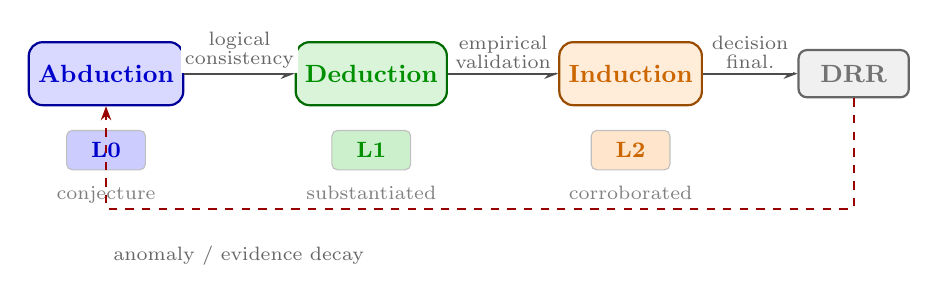
\begin{tikzpicture}[
    node distance=1.6cm and 0.6cm,
    phase/.style={
        draw=#1!60!black, thick, rounded corners=5pt,
        minimum width=1.8cm, minimum height=0.8cm,
        font=\small\bfseries, text=#1!80!black,
        fill=#1!15
    },
    layer/.style={
        draw=gray!50, rounded corners=2pt,
        minimum width=1.0cm, minimum height=0.5cm,
        font=\footnotesize\bfseries, fill=#1!20, text=#1!80!black
    },
    drr/.style={
        draw=gray!80!black, thick, rounded corners=3pt,
        minimum width=1.4cm, minimum height=0.6cm,
        font=\small\bfseries, fill=gray!12, text=gray!90!black
    },
    arr/.style={-{Stealth[length=5pt]}, thick, gray!60!black},
    arrlabel/.style={font=\scriptsize, text=gray!80!black, align=center, fill=white,
        inner sep=1.5pt}
]
    % Phase boxes
    \node[phase=blue] (abd) {Abduction};
    \node[phase=green!70!black, right=1.4cm of abd] (ded) {Deduction};
    \node[phase=orange, right=1.4cm of ded] (ind) {Induction};

    % Layer badges below each phase
    \node[layer=blue, below=0.3cm of abd] (L0) {L0};
    \node[layer=green!70!black, below=0.3cm of ded] (L1) {L1};
    \node[layer=orange, below=0.3cm of ind] (L2) {L2};

    % Layer descriptions
    \node[font=\scriptsize, text=gray, below=0.08cm of L0] {conjecture};
    \node[font=\scriptsize, text=gray, below=0.08cm of L1] {substantiated};
    \node[font=\scriptsize, text=gray, below=0.08cm of L2] {corroborated};

    % Arrows between phases
    \draw[arr] (abd) -- node[arrlabel, above]
        {logical\\[-1pt]consistency} (ded);
    \draw[arr] (ded) -- node[arrlabel, above]
        {empirical\\[-1pt]validation} (ind);

    % DRR box
    \node[drr, right=1.2cm of ind] (drr) {DRR};
    \draw[arr] (ind) -- node[arrlabel, above]
        {decision\\[-1pt]final.} (drr);

    % Feedback loop: DRR back to Abduction
    \draw[arr, dashed, red!60!black]
        (drr.south) -- ++(0,-1.4)
        -| (abd.south);
    % Label centered on the bottom horizontal segment
    \node[arrlabel, fill=white]
        at ($(abd.south)!0.5!(ded.south) + (0,-1.9)$)
        {anomaly / evidence decay};

\end{tikzpicture}

\end{document}